\documentclass[UTF8]{ctexart}
\usepackage{CJK}
\usepackage{amsmath}
\usepackage{amssymb}
\usepackage{graphics}
\usepackage{geometry}
\usepackage{subcaption}
\usepackage{mathrsfs}
\usepackage{pdfpages}
\usepackage{fancyhdr}
\usepackage{placeins}


\pagestyle{plain}

%\setCJKfamilyfont{hei}{黑体}  % 黑体
\newcommand{\hei}{\CJKfamily{hei}}
\newcommand{\xiaoerhao}{\fontsize{18pt}{\baselineskip}\selectfont}
\newcommand{\sihao}{\fontsize{14pt}{\baselineskip}\selectfont}	
\renewcommand{\abstractname}{\xiaoerhao \hei \textnormal{摘 \hspace{3em} 要:}}



\geometry{top=3cm, bottom=3cm, left=2.5cm, right=2.5cm}

\begin{document}
%	\forall i \in N ~ \sum_{k=1}^{K}\sum_{j=1}^{2} X_{ijk}=1
%\end{equation}


%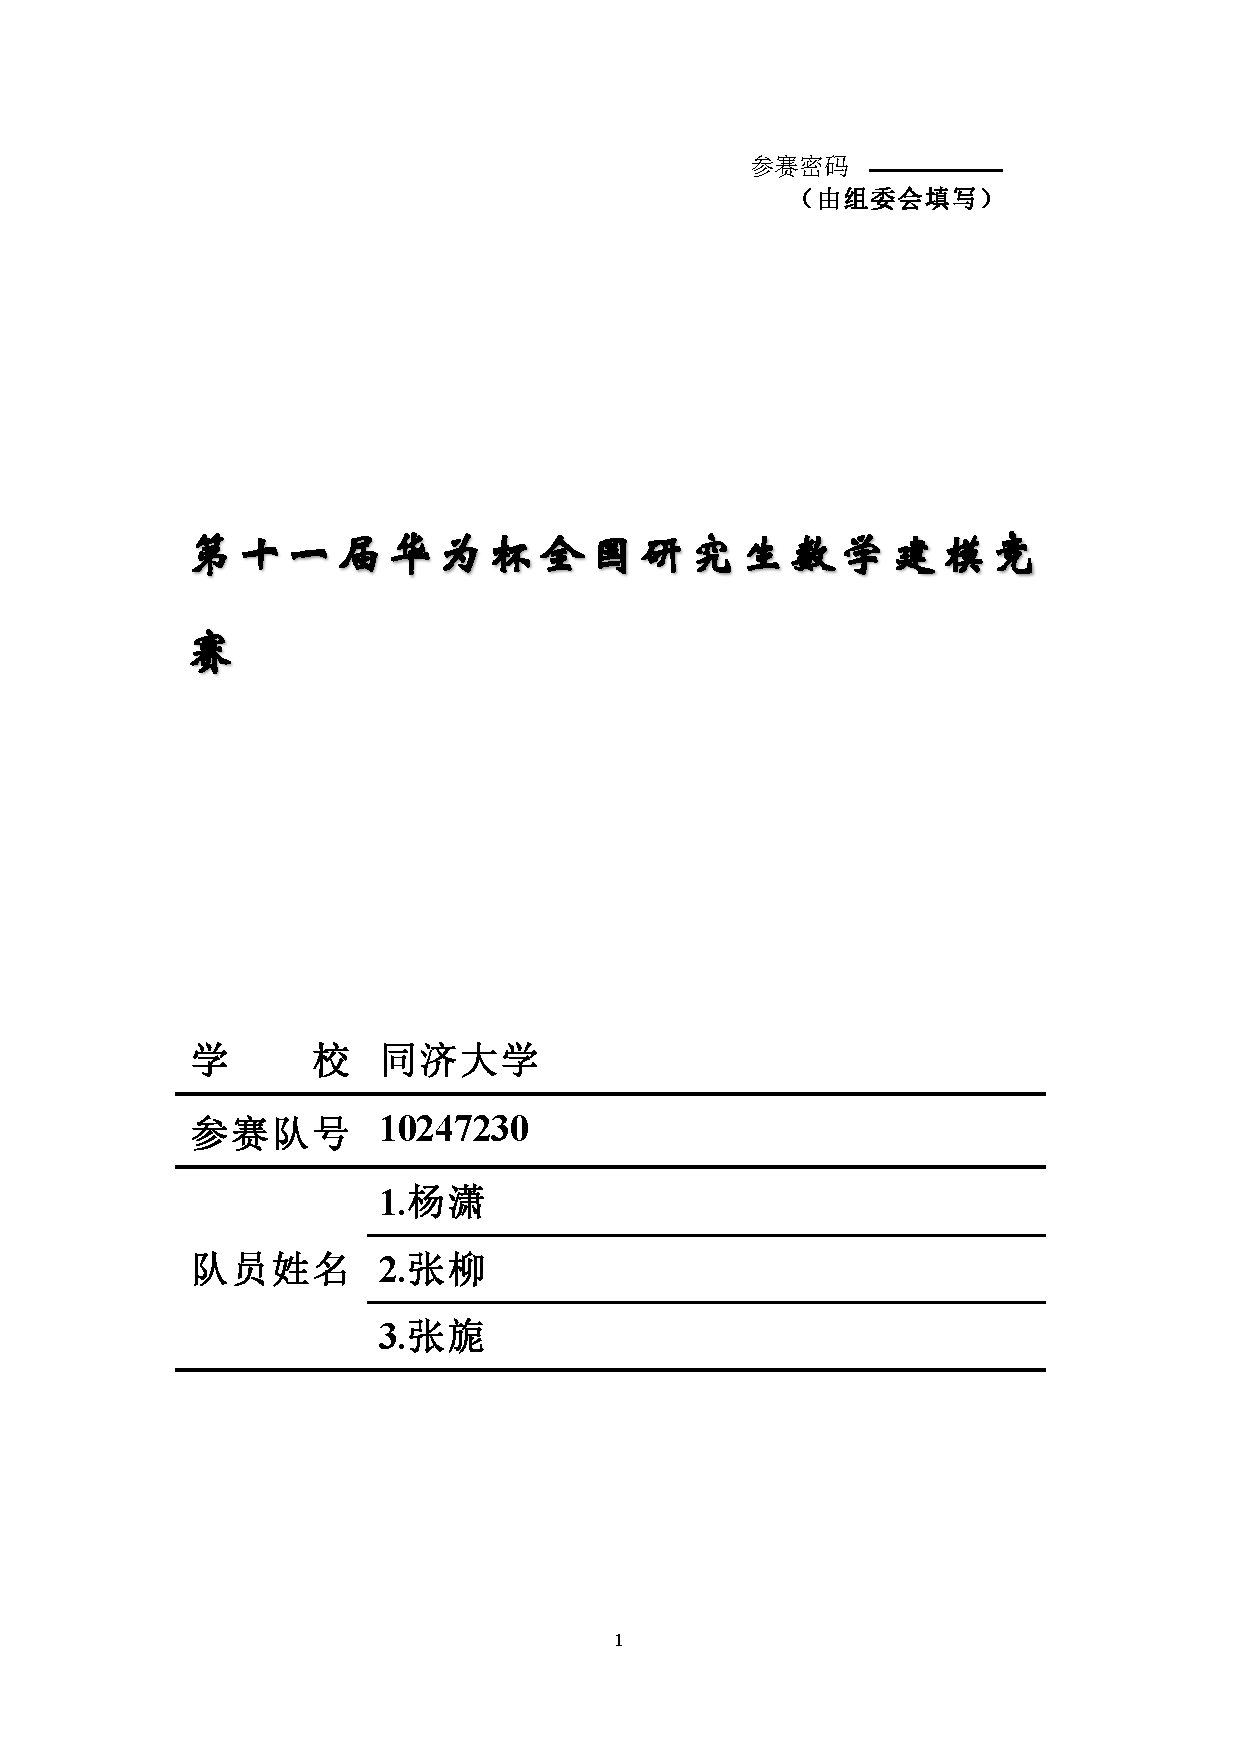
\includepdf{figure/1.pdf} 

\pagebreak
\begin{figure}[t]
	
\includegraphics[width=\linewidth]{figure/header.png}
\end{figure}


\begin{table}[h]
\centering
\begin{tabular}{c  c} 
		{\fontsize{14pt}{\baselineskip}\selectfont 	{题目}} & 
		{\fontsize{16pt}{\baselineskip}\selectfont \textbf{乘用车物流运输计划问题}} \\\cline{2-2}
\end{tabular}

\end{table}

\FloatBarrier

\begin{abstract}
本文对乘用车物流运输计划问题进行了研究,针对不同情境,将问题抽象成不同维度的箱柜装载问题进行建模,并取得了以下几方面的成果。\\

\textbf{针对问题1,2,3:}
主要采用约束编程的建模思想,建立了适用于多种尺寸的乘用车、轿运车的3维乘用车装载数学模型,并获得了在给定乘用车车型数量的前提下,最优的运载分配策略。 \\
结论(1):在题中给定的约束条件下,运载100辆Ⅰ车型的乘用车及68辆Ⅱ车型的乘用车,至少需16辆1-1型乘用车及2辆1-2型乘用车。\\
结论(2):在题中给定的约束条件下,运载72辆Ⅱ车型的乘用车及52辆Ⅲ车型的乘用车,至少需12辆1-1型乘用车及1辆1-2型乘用车。\\
结论(3):在题中给定的约束条件下,运载156辆Ⅰ车型的乘用车及102辆Ⅱ车型的乘用车,至少需25辆1-1型乘用车及5辆1-2型乘用车。\\

\textbf{针对问题4:}
进一步优化了问题1,2,3中的数学模型,完善并支持了考虑行车路线问题的轿运车运输乘用车问题,并给出了通用算法和程序解决了乘用车装载方案及行车路线方案。\\
结论:在题中给定的约束条件及运输路线下,运输166辆Ⅰ车型的乘用车和78辆Ⅱ车型的乘用车至少需22辆1-1型乘用车及4辆1-2型乘用车。\\

\textbf{针对问题5:}
在乘用车、轿运车类型、尺寸、数量、目的地更多样化的情境下,持续优化了问题4中建立的3维乘用车装载模型,以支持复杂的乘用车装载问题的建模和分析需求,并通过经验分析增加了必要的约束条件以缩小解空间,以保证在更短时间内求得较优解。 \\

本文综合运用数理统计、分支限界等数学方法,箱柜装载问题的建模思想,借助Gecode系统建立了多种满足约束编程思想的数学模型,并对所提出问题进行了研究,具有很好的实用性与推广性。最后,总结了模型的优点与不足,为后续研究此类问题的学者提供了一个新的思路。

\end{abstract}

\makeatletter
\def\ckey#1{\def\@ckey{#1}}\def\@ckey{}
\def\makeak{
  \fontsize{14pt}{\baselineskip}\selectfont
  \hspace{0.01em}{关键字:} \@ckey
}
\makeatother

\ckey{约束编程,箱柜装载,轿运车调度}
\makeak
\clearpage
\tableofcontents
\clearpage


\section{问题重述}
\subsection{提出问题}
	近年来我国汽车市场每年平均以25\%的速度快速增长,其发展速度快于国民经济的增长。汽车消费需求的增长,促进了乘用车的整车物流量迅速上升。乘用车生产厂家根据全国客户的购车订单,向物流公司下达运输乘用车到全国各地的任务,物流公司则根据下达的任务制定运输计划并配送这批乘用车。为此,物流公司首先要从他们当时可以调用的“轿运车”中选择出若干辆轿运车,进而给出其中每一辆轿运车上乘用车的装载方案和目的地,以保证运输任务的完成。
但因轿运车、乘用车规格的多样性和运输路线的多样性,当前很多物流公司在制定运输计划时主要依赖调度人员的经验。而在运输任务较复杂时,往往会发生运输效率低下,运输成本不理想等问题。物流公司希望能够在确保完成运输任务的前提下寻求降低运输成本的方法。
“轿运车”是通过公路来运输乘用车整车的专用运输车。本文涉及的双层轿运车分为三种子型:上下层各装载1列乘用车,故记为1-1型(图1);下、上层分别装载1、2列,记为1-2型(图2);上、下层各装载2列,记为2-2型(图3),每辆轿运车可以装载乘用车的最大数量在6到27辆之间。
\begin{figure}[h!]
\begin{minipage}[t]{0.32\textwidth}
  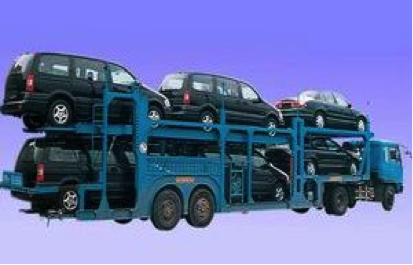
\includegraphics[width=\linewidth]{figure/1-1.png}
  \caption{1-1型轿运车}
\end{minipage}
~
\begin{minipage}[t]{0.32\textwidth}
  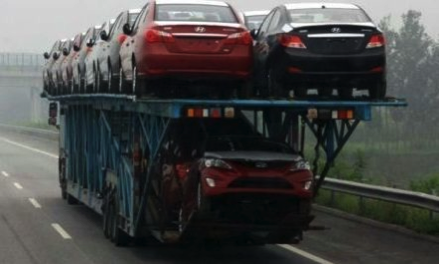
\includegraphics[width=\linewidth]{figure/1-2.png}
  \caption{1-2型轿运车}
\end{minipage}
~
\begin{minipage}[t]{0.32\textwidth}
  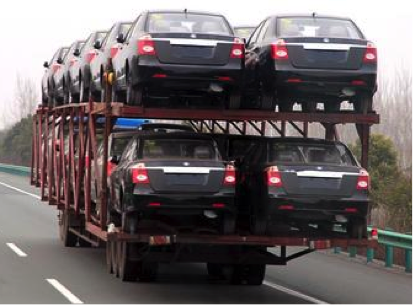
\includegraphics[width=\linewidth]{figure/2-2.png}
  \caption{2-2型轿运车}
\end{minipage}
\end{figure}
%~
%\begin{subfigure}[t]{0.32\textwidth}
%  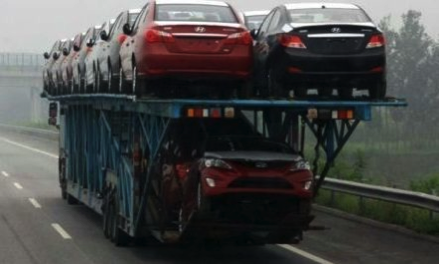
\includegraphics[width=\linewidth]{figure/1-2.png} 
%    \caption{data distribution of \textit{create index}}
%\end{subfigure}
%~
%\begin{subfigure}[t]{0.32\textwidth}
%  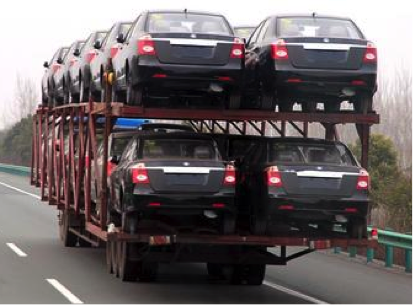
\includegraphics[width=\linewidth]{figure/2-2.png} 
%    \caption{data distribution of \textit{insert table}}
%\end{subfigure}


\subsection{问题要求}
建立数学模型,以通用算法和程序解决整车物流成本优化的问题,能够比较准确得模拟整车物流的装载方案及行车路线,更好地降低整车物流运输成本。本次竞赛需要解决的具体问题如下所述:
问题一:物流公司要运输Ⅰ车型的乘用车100辆及Ⅱ车型的乘用车68辆。
问题二:物流公司要运输Ⅱ车型的乘用车72辆及Ⅲ车型的乘用车52辆。
问题三:物流公司要运输Ⅰ车型的乘用车156辆、Ⅱ车型的乘用车102辆及Ⅲ车型的乘用车39辆。
问题四:物流公司要运输166辆Ⅰ车型的乘用车(其中目的地是A、B、C、D的分别为42、50、33、41辆)和78辆Ⅱ车型的乘用车(其中目的地是A、C的,分别为31、47辆),具体路线见图4,各段长度:OD=160,DC=76,DA=200,DB=120,BE=104,AE=60。
问题五:附件的表1给出了物流公司需要运输的乘用车类型(含序号)、尺寸大小、数量和目的地,附件的表2给出可以调用的轿运车类型(含序号)、数量和装载区域大小(表里数据是下层装载区域的长和宽, 1-1型及2-2型轿运车上、下层装载区域相同;1-2型轿运车上、下层装载区域长度相同,但上层比下层宽0.8米。此外2-2型轿运车因为层高较低,上、下层均不能装载高度超过1.7米的乘用车。

\section{模型假设}
\begin{enumerate}
	\item 	题目中所列数据均真实可靠;
	\item	乘用车与轿运车两侧的安全距离在说明装载区域大小时已经考虑;
	\item	乘用车不可在轿运车上倾斜摆放;
	\item	轿运车运输路线为有向图;
	\item	运输花费主要由轿运车数量决定,次要由轿运车类型决定,最后由轿运车里程数决定。

\end{enumerate}

\section{基本符号说明}
\label{sec:symbols}

	\begin{itemize}
		\item $N$ 乘用车总数
		\item $i$ 乘用车下标, $i \in N$
		\item $K$ 为轿运车使用量
		\item $k$ 轿运车下标,  $k \in K$
		\item $j$ 轿运车层级下标, $j \mapsto \{1,2\}$
		\item $l$ 乘用车长度
		\item $l_i$ 第$i$辆乘用车长度
		\item $w$ 乘用车宽度
		\item $w_i$ 第$i$辆乘用车的宽度
		\item $h$ 乘用车高度
		\item $h_i$ 第$i$辆乘用车的高度
		\item $d$ 乘用车目的地
		\item $d_i$ 第$i$辆的目的地 $d_i \mapsto \{A, B, C, D\}$
		\item $D$ 表示出发地$O$到各目的地的距离, $D=\{D_A, D_B, D_C, D_D\}$
		\item $C$ 运输成本
		\item $C_k$ 第$k$辆轿运车的运输成本
		\item $L$ 轿运车长度
		\item $L_{jk}$ 第$k$辆轿运车第$j$层的长度
		\item $W$ 轿运车宽度
		\item $W_{jk}$ 第$k$辆轿运车第$j$层的宽度
		\item $T$ 轿运车类型
		\item $T_k$ 第$k$辆轿运车的类型, $T_k \mapsto \{1, ~2, ~3 \dots \}$,其中$1$代表1-1型轿运车,$2$代表1-2型轿运车,$3$代表2-2型轿运车
		
		
	\end{itemize}


\section{问题分析}
本文的基本问题是解决如何分配乘用车到轿运车并使整体运输成本最低的问题。
经过对问题本身的分析,
该问题可以视作组合优化问题( Combinatorial Optimization Problem),
而组合优化问题从计算复杂度上来看属于NP-困难问题,即在多项式时间内
无法确定能够找到有效算法求解的问题。

本文拟采用约束编程(Constraint Programming)的思想进行建模与求解。
而对于组合优化的问题,还需列出对应的最大化或者最小化的目标函数。



\subsection{问题一、二、三分析}
问题一、二、三要求计算各种类型轿运车的数量和每辆轿运车的乘用车装载方案,各类型乘用车数量已知,
所需各类型轿运车数量及各轿运车的装载方案未知,但不涉及运输目的地的差异。并且,问题一、二、三
的差异仅为输入参数不同,所以拟建立通用的基于约束编程的模型进行求解。
解决该问题一共有三个关键点:
\begin{itemize}
	\item 采用何种策略将乘用车分配给轿运车;并分配给轿运车的何层。
	\item 对于已分配的乘用车,如何判断是否满足该轿运车层的长宽约束。
	\item 如何构造目标函数。
	\item 采用何种搜索策略能够较快接近并找到最优解。
\end{itemize}
所以建立的基于约束编程的数学模型,主要是解决以上提出的关键问题。
具体的模型建立参考\ref{sec:q123_model}节。




\subsection{问题四分析}
问题四要求在考虑行车路线的情况下解决轿运车运输乘用车问题,计算所需各类型轿运车的数量及每辆轿运车的乘用车装载方案。
各类型乘用车数量已知,所需各类型轿运车数量及各轿运车的装载方案未知。
为解决这一问题,需要在前三题建立的通用模型基础之上,额外考虑运输路线的因素,并添加相关的限制条件。
因为我们假设运输路线是一个有向图,所以只会有O$\rightarrow$D$\rightarrow$C,和O$\rightarrow$D$\rightarrow$B$\rightarrow$A这两条运输路线。
因此,针对路线O$\rightarrow$D$\rightarrow$C,可以约束只有终点是D,C的乘用车可以在一辆轿运车上一次运输。针对路线O$\rightarrow$D$\rightarrow$B$\rightarrow$A,
可以约束只有终点是D,B,A的乘用车可以在一辆轿运车上一次运输。因终点是D的乘用车在这两条路线的轿运车里都可以装载
,因此可以把装载终点是D的乘用车的装载优先级放低。又因行驶路线为有向图,所以在O$\rightarrow$D$\rightarrow$C这一运输路线中,
我们认为终点是C的乘用车的运载优先级高于终点是D的乘用车。同理可得,终点是A的乘用车的运载优先级高于终点是B的乘用车,
而终点是B的乘用车的运载优先级高于终点是D的乘用车。各段长度:OD=160,DC=76,DA=200,DB=120也需要被添加到约束条件里,
以将行使里程考虑在行使成本中,半定量化最终的运输成本。因此,对这一问,可以在解决1-3问的通用数学模型的基础之上,
加上以上这些约束条件以保证满足本题的运载条件,并获得在给定条件下的最优解。\\
为了简化模型的求解,我们对该问题做如下处理:
\begin{itemize}
	\item 在确定分配方案时,限制仅目的地为$\{C,~D\}$或$\{D,~B,~A\}$的组合可以出现在同一轿运车。
	\item 仅在目的地组合相同的分配方案调整车与目的地的映射关系使得总成本在考虑目的地距离的情况下最低。
\end{itemize}


\begin{figure}[h!]
	\centering
	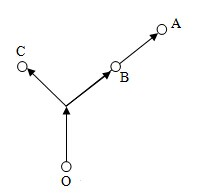
\includegraphics[width=0.3\linewidth]{figure/Q4.png}
	\caption{问题四涉及目的地及其位置关系}
\end{figure}

\subsection{问题五分析}
问题五要求在给定各轿运车、乘用车数量的前提下,综合各车运输路线的情况,解决轿运车运输乘用车的装载问题。。需运输的各类型乘用车数量已知,可使用的轿运车具体型号及数量上限已知,各乘用车运输终点已知,所需各类型轿运车数量及各轿运车的装载方案未知。
为解决这一问题,需要在第四题已建立的通用模型基础之上,额外考虑各具体型号轿运车的数量上限,并添加相关的限制条件。为此我们需要扩展轿运车的类型到一个二维变量,以同时包含其类型及具体型号信息。此外,因为我们依然假设运输路线是一个有向图,所以只会有O->D->C,和O->D->B->A(->E),O->D->B->E这三条到达C,E,A的运输路线。因此,针对路线O->D->C,可以约束只有终点是D,C的乘用车可以在一辆轿运车上一次运输。针对路线O->D->B->A(->E)和O->D->B->E可以约束只有终点是D,E,B,A的乘用车才可以在一辆轿运车上一次运输。因终点是D的乘用车在这两条路线的轿运车里都可以装载,因此可以把装载终点是D的乘用车的装载优先级放低。又因行驶路线为有向图,所以在O->D->C这一运输路线中,我们认为终点是C的乘用车的运载优先级高于终点是D的乘用车。同理可得,终点是E的乘用车的运载优先级高于终点是A的乘用车,而重点是A的乘用车优先级高于终点是B的乘用车,终点是B的乘用车的运载优先级高于终点是D的乘用车。各段长度:OD=160,DC=76,DA=200,DB=120,BE=104,AE=60也需要被添加到约束条件里,以将行使里程考虑在行使成本中,半定量化最终的运输成本。因此,对这一问,可以在解决第四问的通用数学模型的基础之上,加上以上这些约束条件以保证满足本题的运载条件,并获得在给定条件下的最优解。

\begin{figure}[h!]
	\centering
	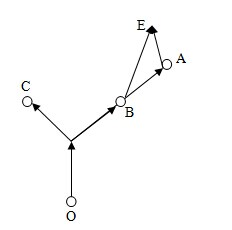
\includegraphics[width=0.3\linewidth]{figure/Q5.png}
	\caption{问题五涉及目的地及其位置关系}
\end{figure}


\section{技术背景}
\subsection{约束编程(Constraint Programming)}
约束编程是一种编程范型,在这种编程范型中,变量之间的关系以约束的形式组织。所谓约束,即指的是一个问题的定义域,问题的描述(约束条件)。一般地,约束编程的支持通用的求解程序对约束模型进行求解。
过程式语言,如C、C++解决问题的方法是通过给出一组机器指令,一步步完成问题的求解。相比之下,约束编程只需声明问题实体之间的关系,具体求解过程是由系统来自动完成的。约束表示了一组实体之间的关系,约束说明列举了当求解一组变量值时必需满足和维持一致的一组约束。负责把约束说明转化成程序的约束转化体制决定满足约束系统的方式。
约束式编程的主要特点有:建模、约束传播和搜索。
约束的一个主要功能就是建模,约束是描述许多应用的一种自然语言。约束式语言包含两个方面,定义和行为,可以被分别处理,一旦定义是正确的,就可以得出他们的行为,通过定义和行为的分离,编程人员可以把精力更多地集中于建模。 
 约束传播被用于两种不同的途径,其一,把一些新的信息加入约束存储中。如加入新约束后,当前的信息和传播结果同以前的信息不一样,那么说明当前约束同已有的约束不一致,应停止当前操作。其二,以自然的方式反映当前决定结果,这种能力常被称为信息传播,传播是对决定立刻反应的重要形式。
约束编程最重要的一个应用是用于解决组合问题,在计划、调度、资源分配等复杂问题上的约束编程都干得很出色。组合问题是指那些解是由一系列独立选择的步骤组成,解的正确性不到最后一个决定作出以前是不可知的,通常每次选择都只有有限的备选方案。
 早期的约束编程应用使用内置的搜索优化方法,如节点一致、弧一致、路径一致算法等,CHIP中实现的就是弧一致算法。实际证明,该算法能很好地解决调度任务、汽车生产线安排序列等问题。
在命令编程语言中,有各种约束编程的类库,如Choco (Java library, free software: X11 style),Emma (Python library, proprietary),Gecode (C++ library, free software: X11 style)等。本文涉及的算法及问题求解过程都是基于Gecode求解器实现的。
\subsection{Gecode}
Gecode\cite{gecode}是一个基于c++实现的约束编程模型求解器,
可用于开发基于约束的系统应用程序,是一个可移植、高效的环境。 Gecode是从根本上进行编程开放,这意味着它可以很容易地与其他系统的接口。它支持新的传播者(如约束的执行情况),
分支策略,和搜索引擎编程。新的变量域可以被编程的效率,在有限域和整数集,拿出Gecode预定义变量相同的水平。


\section{模型的建立与求解}
\subsection{模型建立}
\subsubsection{问题一、二、三通用模型}
\label{sec:q123_model}

\paragraph{模型参数}
	\begin{itemize}
			\item $N$ 乘用车总数,$i$表示第$i$辆乘用车, $i \in \{1 \dots N\}$
			\item $K$ 为轿运车使用量, $k$表示第$k$轿运车下标,  $k \in \{1 \dots K\}$
			\item $j$ 轿运车层级, $j \mapsto \{1,2\}$
			\item $l_i$ 第$i$辆乘用车长度
			\item $w_i$ 第$i$辆乘用车的宽度
			\item $h_i$ 第$i$辆乘用车的高度
			\item $C_k$ 第$k$辆轿运车的运输成本, $C=\sum_{k=1}^{K}C_k$
			\item $L_{jk}$ 第$k$辆轿运车第$j$层的长度
			\item $W_{jk}$ 第$k$辆轿运车第$j$层的宽度
			\item $T_k$ 第$k$辆轿运车的类型, $T_k \mapsto \{1, ~2, ~3\}$	
		\end{itemize}
\paragraph{决策变量}
\label{sec:model1_devar}
\begin{itemize}
	\item $s_k \mapsto \{0,1\}, ~ k \in K$, 若变量$s_k$为1,则表示第$k$辆轿运车已经被使用;
	反之,则第$k$辆轿运车未被使用。
	\item $x_{ijk}\mapsto \{0,1\}, ~ i\in N,~ k \in K,~ j\in \{1,2\}$,若$x_{ijk}$为1,
	则表示第$i$辆乘用车被分配到了第$k$辆轿运车的第$j$层。
\end{itemize}

\paragraph{目标函数}
	本问题的目标是最小化已使用的轿运车的数量,而考虑到题设中
	\textit{当所使用的轿运车数量相同的,优先使用耗油量较少的车},所以在考虑目标函数时,我们采用对每种不同的车型
	赋不同的成本值,即在考虑1-1型,1-2型和2-2型轿运车的情况下,$C_{1-1}$=1,$C_{1-2}$=1.0002,
	$C_{2-2}$=1.0004。通过微调不同车型的对应成本值,可以保证在优化过程中能够首先考虑轿运车的使用数目,
	同时在使用数目相同的情况下使用耗油量更少的轿运车。
	\begin{equation}
		C \ = \ \sum_{k=1}^{K}C_k \cdot s_k
	\end{equation}

\paragraph{约束条件}
\label{sec:q123_cons}
	\begin{itemize}
		\item 只有当轿运车确定为使用状态时才能为其分配乘用车
		\begin{equation}
		 x_{ijk} \leq s_k  \quad 	\forall i,~ j
		\end{equation}
		
		\item 所有乘用车必须被分配给某一轿运车
		\begin{equation}
			\sum_{k=1}^{K} \sum_{j=1}^{2} x_{ijk}=1 \quad \forall i
		\end{equation}
		
		\item 1-2的使用数目不得超过1-1使用数目的20\%
		\begin{equation}
			\sum_{k=1}^{K} \ s_k[T_k=2] \leq 20\% \cdot \sum_{k=1}^{K}  \ s_k[T_k=1]
		\end{equation}
		
		\item 对于高度超过1.7米的乘用车,只能放在1-1或1-2型轿运车的下层
		\begin{equation}
			\forall i \ h_i>1.7 \ \implies \sum_{k=1}^{K}x_{i1k}=0
		\end{equation}
		
		\item 对于任一轿运车的任一层,所包含的乘用车必须能够满足该区域的长宽要求
		\begin{align}
		&	\forall k, j \quad  x_{ijk}=1  \implies \notag\\
		&		 cumulatives(W_{jk}, \{xcoord_i | x_{ijk}=1 \},\{ w_i | x_{ijk}=1\},  \{xcoord_i | x_{ijk}=1 \}, \{l_i | x_{ijk}=1\}, L_{jk}) 
		\end{align}
		
		
	\end{itemize}

\paragraph{cumulative约束}
在约束编程的范型中,cumulative约束是一类可以解决在一定资源情限制清况下任务分配的约束。
任务用4-元组\textit{(起始时间,持续时间,终止时间,占用资源)}表示,而资源用2-元组\textit{(资源,限制)}表示。
对于给定的任务集合$\mathscr{T}$,在单资源的情况下,cumulative约束强制在任一时间点,
任务所占的资源数不超过所限制的阈值,单资源情况下cumulative约束所适用的问题如图\ref{fig:cumulative}所示。\\
\begin{figure}[h!]
	\centering
	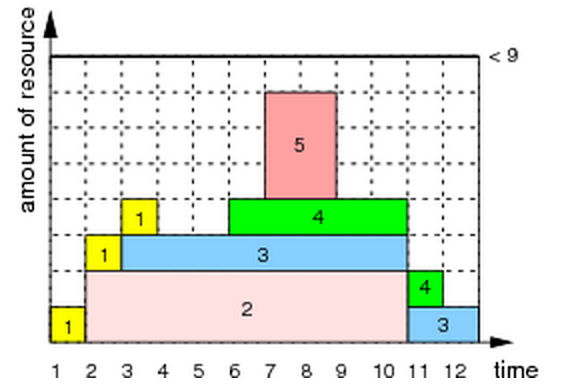
\includegraphics[width=0.4\linewidth]{figure/cumulative.png}
	\caption{cumulative约束}
	\label{fig:cumulative}
\end{figure}

而对于多资源的情况,即对一组资源$\mathscr{R}$和一组任务$\mathscr{T}$,任务必须被
分配到可用的资源并且对各资源的使用不超过资源的限制。定义多资源情况下的cumulative
约束原型如下: 
	\begin{align*}
	cumulatives( resource, start, duration, end, height, limit)
	\end{align*}
根据\cite{cumulatives}中所述思想,我们采用了基于\textit{交换}的cumulatives约束实现,具体算法如
图\ref{al1_cum}和图\ref{al2_cum}所示:

\begin{figure}[h!]
	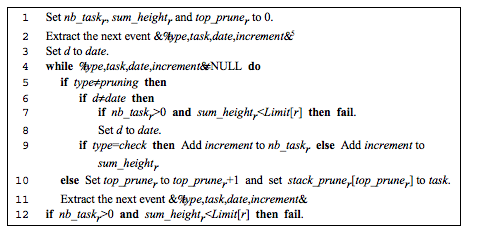
\includegraphics[width=\linewidth]{figure/al1_cum.png}
	\caption{交换算法1}
	\label{al1_cum}
\end{figure}

\begin{figure}[h!]
	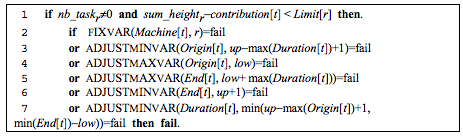
\includegraphics[width=\linewidth]{figure/al2_cum.png}
	\caption{交换算法2}
	\label{al2_cum}
\end{figure}

\begin{figure}[h!]
	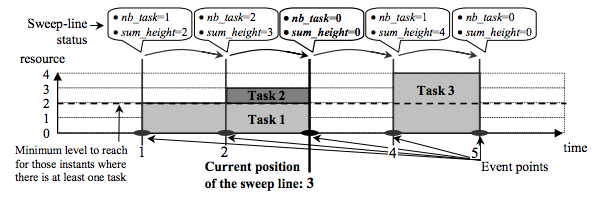
\includegraphics[width=\linewidth]{figure/illustrative_cum.png}
	\caption{交换算法示例}
	\label{ill_cum}
\end{figure}

\paragraph{搜索策略}
为了在解空间的搜索过程中不断最小化目标函数寻找最优解,本问题采用分支定界法(Branch and Bound)\cite{bbalgorithm}来寻找模型的最优解。

它是由R.J.达金和兰德-多伊格在20世纪60年代初提出的。
分支定界法的基本思想是对有约束条件的最优化问题的所有可行解(数目有限)空间进行搜索。
所谓“分支”是采用广度优先的策略,依次生成扩展结点的所有分支(即:儿子结点)。
所谓“限界”是在结点扩展过程中,计算结点的上界(或下界),边搜索边减掉搜索树的某些分支,从而提高搜索效率。
该算法在具体执行时,把全部可行的解空间不断分割为越来越小的子集(称为分支),
并为每个子集内的解的值计算一个下界或上界(称为定界)。
在每次分支后,对凡是界限超出已知可行解值的那些子集不再做进一步分支。
这样,解的许多子集(即搜索树上的许多结点)就可以不予考虑了,从而缩小了搜索范围。
这一过程一直进行到找出可行解为止,该可行解的值不大于任何子集的界限,因此这种算法一般可以求得最优解。\\

分枝界限法是组合优化问题的有效求解方法,其步骤如下所述:
\begin{itemize}
		\item 步骤一:如果问题的目标为最小化,则设定目前最优解的值Z=$\infty$
		\item 步骤二:根据分枝法则(Branching rule),从尚未被洞悉(Fathomed)节点(局部解)中选择一个节点,并在此节点的下一阶层中分为几个新的节点。
		\item 步骤三:计算每一个新分枝出来的节点的下限值(Lower bound,LB)
		\item  步骤四:对每一节点进行洞悉条件测试,若节点满足以下任意一个条件,则此节点可洞悉而不再被考虑:此节点的下限值大于等于Z值。已找到在此节点中,具最小下限值的可行解;若此条件成立,则需比较此可行解与Z值,若前者较小,则需更新Z值,以此为可行解的值。此节点不可能包含可行解。
		\item 步骤五:判断是否仍有尚未被洞悉的节点,如果有,则进行步骤二,如果已无尚未被洞悉的节点,则演算停止,并得到最优解。
\end{itemize}


\subsubsection{问题四模型}
	相较于问题一的模型参数,由于问题四引入了目的地和距离信息,所以问题四的模型基于问题一、二、三
	的通用模型做了在考虑目的地和距离信息情况的扩展。\\
	
	在模型参数部分加入了$d_i$以表示第$i$辆乘用车的目的地。
	根据题设已知OD=160, DC=76, DA=200, DB=120,且该题所设计始发地均为点O,
	由此可以计算出始发地O到各目的地A、B、C、D的距离,距离集合
	$D=\{D_A=360, D_B=280, D_C=216, D_D=160\}$也作为问题四模型的扩展参数。\\
	
	增加决策变量$dest_k$表示第$k$辆车所去的目的地。
	
	问题分析中所提及的两个关键点:
	\begin{enumerate}
		\item 在确定分配方案时,限制仅目的地为$\{C,~D\}$或$\{D,~B,~A\}$的组合可以出现在同一轿运车。
		\item 仅在目的地组合相同的分配方案调整车与目的地的映射关系使得总成本在考虑目的地距离的情况下最低。
	\end{enumerate}
	分别采用增加约束和调整目标函数的方式来实现。
	
	
	
\paragraph{模型参数}
	\begin{itemize}
			\item $N$ 乘用车总数,$i$表示第$i$辆乘用车, $i \in \{1 \dots N\}$
			\item $K$ 为轿运车使用量, $k$表示第$k$轿运车下标,  $k \in \{1 \dots K\}$
			\item $j$ 轿运车层级, $j \mapsto \{1,2\}$
			\item $l_i$ 第$i$辆乘用车长度
			\item $w_i$ 第$i$辆乘用车的宽度
			\item $h_i$ 第$i$辆乘用车的高度
			\item $C_k$ 第$k$辆轿运车的运输成本, $C=\sum_{k=1}^{K}C_k$
			\item $L_{jk}$ 第$k$辆轿运车第$j$层的长度
			\item $W_{jk}$ 第$k$辆轿运车第$j$层的宽度
			\item $T_k$ 第$k$辆轿运车的类型, $T_k \mapsto \{1, ~2, ~3\}$
			\item $d_i$ 第$i$辆车的目的地,$d_i \mapsto \{A, B, C, D\}$		
			\item 出发地$O$到各目的地的距离所在集合为 $D=\{D_A=360, D_B=280, D_C=216, D_D=160\}$
		\end{itemize}
\paragraph{决策变量}
	\begin{itemize}
		\item $s_k \mapsto \{0,1\}, ~ k \in K$, 若变量$s_k$为1,则表示第$k$辆轿运车已经被使用;
		反之,则第$k$辆轿运车未被使用。
		\item $x_{ijk}\mapsto \{0,1\}, ~ i\in N,~ k \in K,~ j\in \{1,2\}$,若$x_{ijk}$为1,
		则表示第$i$辆乘用车被分配到了第$k$辆轿运车的第$j$层。
		\item $dest_k \mapsto \{A,B,C,D\}  ~ k \in K$ $dest_k$表示第$k$辆轿运车被分配的目的地。
	\end{itemize}
\paragraph{目标函数}
			\begin{equation}
				C \ = \ \sum_{k=1}^{K}C_k \cdot s_k
			\end{equation}
	
\paragraph{约束条件}
	\begin{itemize}
		\item 只有当轿运车确定为使用状态时才能为其分配乘用车
		\begin{equation}
		 x_{ijk} \leq s_k  \quad 	\forall i,~ j
		\end{equation}
		
		\item 所有乘用车必须被分配给某一轿运车
		\begin{equation}
			\sum_{k=1}^{K} \sum_{j=1}^{2} x_{ijk}=1 \quad \forall i
		\end{equation}
		
		\item 1-2的使用数目不得超过1-1使用数目的20\%
		\begin{equation}
			\sum_{k=1}^{K} \ s_k[T_k=2] \leq 20\% \cdot \sum_{k=1}^{K}  \ s_k[T_k=1]
		\end{equation}
		
		\item 对于高度超过1.7米的乘用车,只能放在1-1或1-2型轿运车的下层
		\begin{equation}
			\forall i \ h_i>1.7 \ \implies \sum_{k=1}^{K}x_{i1k}=0
		\end{equation}
		
		\item 对于任一轿运车的任一层,所包含的乘用车必须能够满足该区域的长宽要求
		\begin{align}
		&	\forall k, j \quad  x_{ijk}=1  \implies \notag\\
		&		 cumulatives(W_{jk}, \{xcoord_i | x_{ijk}=1 \},\{ w_i | x_{ijk}=1\},  \{xcoord_i | x_{ijk}=1 \}, \{l_i | x_{ijk}=1\}, L_{jk}) 
		\end{align}
		
		\item 限制仅目的地为$\{C,~D\}$或$\{D,~B,~A\}$的组合可以出现在同一轿运车
		%\begin{equation}
			
		%\end{equation}
		
		\item 优先级为$D >_{priority} C$, $A >_{priority} B >_{priority} C $
			\footnote{此次所指优先级应理解为若一辆轿运车同时载有去目的地$C$和$D$,则将轿运车的目的地视为$C$,对于$A,~B,~C$亦同}
		\begin{equation}
			\forall i,k \  x_{ijk}=1 \Leftrightarrow 	dest_k \ \geq_{priority} \ d_i
		\end{equation}
		
	\end{itemize}

\subsubsection{问题五模型}

\subsection{模型求解}
本文所有涉及模型均采用Gecode\cite{gecode}求解

基于上文所介绍的数学模型,我们使用C++建立了数学模型,并对问题进行了求解,本章我们将对问题的答案进行详细的解释说明。

\subsubsection{问题一、二、三求解}
\paragraph{问题一求解}

如表 \ref{tab:answer1}所示,针对问题一,运送100辆I型乘用车以及68辆II型乘用车,我们模型求解得到的最优结果是,使用16辆1-1型轿运车以及2辆1-2型轿运车。相应的装车方案见表\ref{tab:answer1}。实际输出的csv文件格式是横向排列的,由于文档格式的限制,本文档对所有的输出答案进行了格式的更改,我们保证答案是一致的,只是将横向表格更改为了纵向表格,此处理适用于本章的所有输出答案表格,以下将不再对格式更改进行说明。表\ref{tab:answer1}中,第一行展示了运输使用的轿运车类型,第二行展示了使用相同类型,相同装载方式的轿运车数量,其中,相同装载方式意味着在乘用车数量以及位置在这些轿运车中是相同的。从第三行到第八行,展示了乘用车在一辆轿运车中的分布情况,包括在轿运车上层的乘用车数量以及在轿运车下层的乘用车数量。针对1-2型的轿运车上层,装载方式满足对称装载的需求,以左一辆,右一辆的方式进行装载。第九行以及第十行主要是为了第四问而设计的,为保证程序的通用性,虽然前三问没有用到这两项,我们还是对他们进行了输出,在前三问中这两项对于所有的轿运车都采取置零处理。

\begin{table}[h!]
\centering
\caption{问题一分配方案详解}\label{tab:answer1}
\begin{tabular}{|c|c|c|c|c|c|c|}
\hline
轿用车类型 & 1-1 & 1-2 & 1-1 & 1-2 & 1-1 & 1-1\\ \hline 
相同类型、相同装载方式的车辆数 & 5 & 1 & 5 & 1 & 5 & 1\\ \hline 
装在上层序号为1乘用车数量 & 4 & 10 & 4 & 0 & 0 & 0\\ \hline 
装在上层序号为2乘用车数量 & 0 & 0 & 0 & 12 & 5 & 1\\ \hline 
装在上层序号为3乘用车数量 & 0 & 0 & 0 & 0 & 0 & 0\\ \hline 
装在下层序号为1乘用车数量 & 4 & 5 & 4 & 5 & 0 & 0\\ \hline 
装在下层序号为2乘用车数量 & 0 & 0 & 0 & 0 & 5 & 5\\ \hline 
装在下层序号为3乘用车数量 & 0 & 0 & 0 & 0 & 0 & 0\\ \hline 
中间停靠地 & 0 & 0 & 0 & 0 & 0 & 0\\ \hline 
目的地 & 0 & 0 & 0 & 0 & 0 & 0\\ \hline
\end{tabular}
\end{table}


\paragraph{问题二求解}
针对问题二,运送72辆II型乘用车以及52辆III型乘用车,我们模型求解得到的最优结果是,使用12辆1-1型轿运车以及1辆1-2型轿运车来执行此次运输。具体乘用车在轿运车的分布情况详见表\ref{tab:answer2}。表中各项指标均与问题一中的相同,此处不再赘述。
\begin{table}[h!]
\centering
\caption{问题二分配方案详解}\label{tab:answer2}
\begin{tabular}{|c|c|c|c|c|c|}
\hline
轿用车类型 & 1-1 & 1-2 & 1-1 & 1-1 & 1-1\\ \hline 
相同类型、相同装载方式的车辆数 & 5 & 1 & 5 & 1 & 1\\ \hline 
装在上层序号为1乘用车数量 & 0 & 0 & 0 & 0 & 0\\ \hline 
装在上层序号为2乘用车数量 & 5 & 12 & 5 & 5 & 4\\ \hline 
装在上层序号为3乘用车数量 & 0 & 0 & 0 & 0 & 0\\ \hline 
装在下层序号为1乘用车数量 & 0 & 0 & 0 & 0 & 0\\ \hline 
装在下层序号为2乘用车数量 & 0 & 0 & 0 & 0 & 1\\ \hline 
装在下层序号为3乘用车数量 & 4 & 5 & 4 & 4 & 3\\ \hline 
中间停靠地 & 0 & 0 & 0 & 0 & 0\\ \hline 
目的地 & 0 & 0 & 0 & 0 & 0\\ \hline 
\end{tabular}
\end{table}


\paragraph{问题三求解}
针对问题三,运送156辆I型乘用车、102辆II型乘用车以及39辆III型乘用车,我们模型求解得到的最优结果是,使用25辆1-1型轿运车以及5辆1-2型轿运车来完成这个运输任务。表\ref{tab:answer3}详细介绍了乘用车在轿运车中的分配方案,表中各项指标均与问题一种的相同,如表中有不明确的地方,请参照问题一中的表中的指标说明。
\begin{table}[h!]
\centering
\caption{问题三分配方案详解}\label{tab:answer3}
\begin{tabular}{|c|c|c|c|c|c|c|c|c|c|c|c|c|c|}
\hline
轿用车类型 & 1-1 & 1-2 & 1-1 & 1-1 & 1-2 & 1-1 & 1-2 & 1-1 & 1-2 & 1-1 & 1-1 & 1-1 & 1-2\\ \hline 
相同类型、相同装载方式的车辆数 & 5 & 1 & 4 & 1 & 1 & 5 & 1 & 5 & 1 & 1 & 1 & 3 & 1\\ \hline 
装在上层序号为1乘用车数量 & 4 & 4 & 4 & 4 & 4 & 4 & 4 & 4 & 4 & 4 & 0 & 0 & 0\\ \hline 
装在上层序号为2乘用车数量 & 0 & 8 & 0 & 0 & 8 & 0 & 8 & 0 & 8 & 0 & 5 & 5 & 12\\ \hline 
装在上层序号为3乘用车数量 & 0 & 0 & 0 & 0 & 0 & 0 & 0 & 0 & 0 & 0 & 0 & 0 & 0\\ \hline 
装在下层序号为1乘用车数量 & 0 & 0 & 0 & 3 & 2 & 4 & 2 & 4 & 2 & 4 & 3 & 0 & 0\\ \hline 
装在下层序号为2乘用车数量 & 0 & 4 & 0 & 0 & 4 & 0 & 4 & 0 & 4 & 0 & 1 & 5 & 6\\ \hline 
装在下层序号为3乘用车数量 & 4 & 2 & 4 & 1 & 0 & 0 & 0 & 0 & 0 & 0 & 0 & 0 & 0\\ \hline 
中间停靠地 & 0 & 0 & 0 & 0 & 0 & 0 & 0 & 0 & 0 & 0 & 0 & 0 & 0\\ \hline 
目的地 & 0 & 0 & 0 & 0 & 0 & 0 & 0 & 0 & 0 & 0 & 0 & 0 & 0\\ \hline 
\end{tabular}
\end{table}

\subsubsection{问题四求解}
针对问题四,运送42辆I型乘用车以及31辆II型乘用车到A地,50辆I型乘用车到B地,33辆I型乘用车以及47辆II型乘用车到C地,41辆I型乘用车到D地的问题,我们模型求解的最优结果是,使用6辆直接开往A地的1-1型轿运车,1辆直接开往A地的1-2型轿运车以及1辆中途停留B地,最终开往A地的1-1型轿运车;使用3辆直接开往B地的1-1型轿运车,1辆直接开往B地的1-2型轿运车以及1辆中途停留D地,最终目的地B地的1-1型轿运车;使用7辆直接开往C地的1-1型轿运车以及1辆直接开往C地1-2型轿运车;使用4辆直接开往D地的1-1型轿运车以及1辆直接开往D地的1-2型轿运车。所有轿运车运输的总里程数为6968,其中1-1型轿运车的里程为5932,1-2型轿运车的里程为1036。详细的轿运车装载乘用车运输方案见表\ref{tab:answer4}。第四文中,输出项,最后两项中间停靠地以及目的地均被使用,中间停靠地意味着该轿运车需要在此地卸一部分货,如果轿运车不需要在中间地卸货,我们就将中间停靠地置为零,虽然轿运车仍然途径其他一些地方,但是这些轿运车不需要在中途卸货。中间停靠地即为中间卸货地。
\begin{table}[h!]
\centering
\caption{问题四分配方案详解}\label{tab:answer4}
\begin{tabular}{|c|c|c|c|c|c|c|c|c|c|c|c|c|c|}
\hline
轿用车类型 & 1-1 & 1-1 & 1-2 & 1-1 & 1-1 & 1-2 & 1-1 & 1-1 & 1-2 & 1-1 & 1-1 & 1-2 & 1-1\\ \hline 
相同类型、相同装载方式的车辆数 & 5 & 1 & 1 & 1 & 3 & 1 & 1 & 4 & 1 & 3 & 3 & 1 & 1\\ \hline 
装在上层序号为1乘用车数量 & 4 & 0 & 2 & 4 & 4 & 10 & 4 & 4 & 1 & 0 & 4 & 10 & 0\\ \hline 
装在上层序号为2乘用车数量 & 0 & 5 & 10 & 0 & 0 & 0 & 0 & 0 & 11 & 5 & 0 & 0 & 0\\ \hline 
装在下层序号为1乘用车数量 & 4 & 0 & 0 & 0 & 4 & 5 & 4 & 4 & 0 & 0 & 4 & 5 & 1\\ \hline 
装在下层序号为2乘用车数量 & 0 & 5 & 6 & 5 & 0 & 0 & 0 & 0 & 6 & 5 & 0 & 0 & 0\\ \hline 
中间停靠地 & 0 & 0 & 0 & B & 0 & 0 & D & 0 & 0 & 0 & 0 & 0 & 0\\ \hline 
目的地 & A & A & A & A & B & B & B & C & C & C & D & D & D\\ \hline 
\end{tabular}
\end{table}


\subsubsection{问题五求解}
本模型是基于约束编程的思想所建立,由于第五题问题相对复杂,需要使用较多的约束,编写这些复杂的约束也是一件复杂的任务,由于本次比赛时间所限,约束编程是一个较新的,较复杂的建模,编程思想,我们接触的时间也不是很长,对此并不是十分精通,因此,在提交最终作品时,我们并没有完成全部约束条件的编写,我们不能解决如第五题一样复杂的乘用车分配以及运输问题。这是一个非常有趣的问题,我们会继续完善此编程。基于对约束编程的研究,我们有理由认为,使用约束编程来解决此类问题,可以保证在最短的时间内得到问题的最优解,其求解效率高于一般普通算法对此类问题的求解。约束编程在建模以及解模型领域有广阔的前景。

\section{模型的评价、改进及推广}
本文分别对乘用车、轿运车装载方式进行了建模求解,在数据简单解空间较小的情况下计算获得了问题的最优解;在数据复杂解空间过大无法求解的情况下,也根据实际情况为模型设置了约束条件,缩小了解空间。该模型若能继续完善,深入推广,将极大程度上改善物流公司的调度机制,为公司缩减物流成本,提高运输效率提供有力支持。在建模过程中,我们的模型得到了验证,但也不能忽视所存在需要改进的问题,现分析如下:
\begin{itemize}
     \item	本模型借助了Gecode求解器通用模型框架实现,该框架内的算法性能虽然已经较优,但整体上受框架约束较大。目前的约束实现是基于Gecode提供的通用传播者(propagator)和分支程序(brancher),所以该模型的求解效率可以通过自定义领域相关的传播者和分支程序来进一步提高。而对于多资源的情况,即对一组资源R和一组任务T ,任务必须被分配到可用的资源并且对各资源的使用不超过资源的限制。如希望进一步优化提高运算效率,需改造Gecode求解器内部算法,但这样在具体实现上将较为繁琐。\\
     \item在问题四中,目前得到的结果可能是一个最优解也可能只是一个较优解。因目前的模型中的约束条件还未全部完善起来,会导致解空间较大的问题产生。在固定时间内仅能得到一个较优解。后续我们也将继续完善这一部分模型,力求获得更优质的装配方案推荐。\\
      \item	在问题五中,现虽已针对题中提供的信息完成建模,但很遗憾因时间关系暂未完全实现。
今后努力方向:
\end{itemize}


我们将继续深化对乘用车、轿运车装载问题的研究,自定义领域相关的传播者和分支程序来进一步提高现有的运算效率,在一定解空间范围内更快得到最优结果。希望能够做出更加深入、扎实、优质的研究成果,以解决物流公司在乘用车运载调配方面的难题。





\begin{thebibliography}{1}  % even better: use BibTeX!
\bibitem{gecode} Gecode Team.  \textit{Gecode}: Generic Constraint
  Development Environment, 2006. 
  
\bibitem{cumulatives}Beldiceanu, Nicolas, and Mats Carlsson. "A new multi-resource cumulatives constraint with negative heights." Principles and Practice of Constraint Programming-CP 2002. Springer Berlin Heidelberg, 2002. 

\bibitem{bbalgorithm} Land, Ailsa H., and Alison G. Doig. "An automatic method of solving discrete programming problems." Econometrica: Journal of the Econometric Society (1960): 497-520.

%\bibitem{Search} Simonis, Helmut, and Barry O’Sullivan. "Search strategies for rectangle packing." \emph{Principles and Practice of Constraint Programming.} Springer Berlin Heidelberg, 2008.

\end{thebibliography}

\appendix
\section{代码}




\end{document}